\section{Pauli component erasing maps}
\label{sec:pce_maps}
% \janote{Propuesta: hacer un switch de títulos entre el título de II y de II.B}
% \janote{En este primer agregué las referencias a en cuáles secciones hablamos de qué}
% To introduce in \ref{sec:single:qubit} the family of Pauli component erasing 
% maps we start in \ref{subsec:qtm_ch} reviewing basic concepts of quantum 
% channels that will allow us to introduce some notation. 

% \afnote{Propongo que cambiemos el inicio de esta sección por: 
In this section we introduce the family of Pauli component erasing (PCE)
maps. Let us start our discussion with a brief review of several basic concepts
of quantum channels that will allow us to introduce some notation, 
and finish with the definition of PCE maps, some generalities. We further 
introduce a useful graphical representation  for them.
% of the aforementioned maps. 
% and finish with the definition of PCE maps, some generalities and a graphical representation. 
% }
% In this section we introduce the definition of Pauli component erasing maps,
% but first we go through several standard definitions needed to discuss them.
\subsection{Quantum channels} \label{subsec:qtm_ch}% {{{
% \afnote{Creo que podríamos empezar la sección introduciendo el espacio de
% Hilbert y esas cosas y después si dedicarse solamente a Quantum channels. Si
% están de acuerdo, entonces sólo tendriamos que cambiar el orden de las dos
% primeras frases en el primer párrafo.}
Quantum channels are the most general linear operations that a quantum system
undergo independently of its past~\cite{zimansbook,cirac}.  The physical system
under study will be associated with a Hilbert space denoted by \hilbert{}, and
the set of linear operators over such space will be denoted by
$\mcB(\hilbert)$. That way, a density matrix $\rho$ of such system is an
element of $\mcB(\hilbert)$.
% \afnote{En esta última parte podriamos cambiar asi:}
% \afnote{The state of the physical system under study is associated to a
% Hilbert space \hilbert{}, and the set of linear operators over such space is
% denoted by $\mcB(\hilbert)$. In this way, a density matrix $\rho$ of such
% system is an element of $\mcB(\hilbert)$.}
% Quantum channels comprehend the most general linear operations that a quantum
% system undergo independently of its past~\cite{zimansbook,cirac}. To introduce
% their construction and properties, first let us define several objects. We will
% denote Hilbert spaces as \hilbert and $d$-dimensional Hilbert spaces as
% $\hilbert_d$. The set of linear operators over a Hilbert space \hilbert will
% be written as $\mcB(\hilbert)$, and the set of density operators as $\mcS(\hilbert)$.
%, the subset of density matrices as
%$\mcS(\hilbert)$, which is in turn a subset of the so called trace-class
%operators $\mcT(\hilbert)$, for the finite dimensional case, the one studied
%here, $\mcT(\hilbert)$ and $\mcB(\hilbert)$ coincide~\cite{zimansbook}. 

The construction of quantum channels includes basically three ingredients:
linearity, trace preservation and complete positivity. Linearity is needed to
map every convex combination of density matrices into a convex combination of the
evolution of such density matrices. The
trace preserving property is required for the process $\mcE$ 
 to happen with probability $1$, and reads $\tr\mcE[\rho]=\tr \rho =1$. 
Often, this condition is easy to test.
The
complete
positivity condition is needed to preserve positive semidefiniteness and handle
the non-local nature of quantum theory.
A linear map $\mcE$ is positive if it maps density operators to density operators, \ie{}
if $\mcE[\rho]\geq 0$ for all density matrices $\rho$. 
% 
% $\mcE[\Delta]\geq 0 \ \ \forall \Delta \in \mcB(\hilbert)$ hermitian with $\Delta\geq 0$\cpnote{Francois, de tu nota, la $\Delta$ ya es hermitica, pues 
% decimos que es una matriz de densidad} \ddnote{Aqui hablamos de matrices
% positivas definidas en general, estuve revisando en varios libros, y parece que
% lo mas estandar es suponer que si se dice que es positiva (o negativa) definida
% o semi-definida, automaticamente se dice que es hermítica. Sin embargo hay
% definiciones mas generales que involucran matrices no hermiticas, esas eran las
% que yo tenía en mente (pero parece que no son tan conocidas). Opto por
% mencionar que $\Delta$ es hermítico.}. 
%
On the other hand, if one extends a positive map to include an ancilla, the resulting
map is not always positive. If, for an ancillary system of arbitrary dimension, such extension
results in a positive map, we say that the original map is completely
positive~\cite{bengtsson_zyczkowski_2017}.
Quantum channels are required to be completely positive
so as to allow the proper evolution of potentially entangled states with an
ancilla; to test this condition we require some additional steps. 
% \afnote{Sería bueno mencionar también que la tarea de determinar la CP
% de un mapa es no trivial, lo que sirviría también como conector o preambulo del
% siguiente párrafo.}
% In the other hand, a map is completely positive if extending the 
%  $\id_k \otimes \mcE$ is a positive map for $k=1,2,\dots$, where $\id_k$ is the identity channel over $\mcB(\hilbert_k)$. This ensures that every positive semidefinite operator of any
% extension of the system (where the quantum channel is now a local operation) is
% mapped to a positive semidefinite operator. The trace preserving is automatically
% fulfilled for all extensions if $\mcE$ fulfills it. Therefore, any density matrix of a system
% where $\mcE$ acts locally, is sent to a valid density matrix, this is the
% substance of complete positivity.
% \flnote{No creo que lo de Bell state sea conveniente. Mejor decir algo como: E
% is totally positive if trivially extending E to the tensor product of H with an
% arbitrary dimensional ancilla space yields a positive operation.
% }\ddnote{ejecutado} 
% Concluding, quantum channels are linear completely positive trace preserving
% maps.

A simple algorithm to test the complete positivity of a quantum channel 
was developed by 
\jami{}~\cite{jamil} and Choi~\cite{choi}.
One first exploits an isomorphism that maps a channel $\mcE$ to the state
$\choi=\left(\id \otimes \mcE\right)[\proj{\Omega}{\Omega}]$, where
$\ket{\Omega}=1/\dim(\hilbert)\sum_i^{\dim(\hilbert)}\ket{i}\ket{i}$ is a 
maximally entangled state between the original system and an ancilla and
``$\id$'' is the identity channel.
Remarkably, the map \mcE{} is completely positive
if and only \choi{} (also called Choi or dynamical matrix of $\mcE$) 
is positive-semidefinite~\cite{jamil,choi}. 
% \afnote{No sé si es algo obvio, pero creo que seria bueno comentar que es el objeto $\id$.}
%  the
% Bell state between two copies of \hilbert. 

% }}}
\subsection{Structure of PCE maps} % {{{
\label{sec:single:qubit}
% \todo{David escribe una primera version y luego Carlos itera}
% Now that we have discussed the main features of quantum channels
% we are going to introduce the Pauli component erasing maps.
% We shall start exploring the single qubit scenario 
% and continue with the $N$-qubit case. 
% 
% \afnote{
We have discussed the main features of quantum channels, now
we turn our attention to introduce the Pauli component erasing maps. We start
by exploring the single qubit scenario and then we treat the $N$-qubit case.
% }

The most general single qubit density matrix can be written as
\begin{equation}
% \rho=\frac{\one +\vec r \cdot \vec \sigma}{2}.
\rho=\frac12 {\sum_{\alpha=0}^3 r_\alpha \sigma_\alpha},
\end{equation}
% \afnote{Creo que este párrafo queda mejor así: where
% $\{\sigma_{0},\sigma_{1},\sigma_{2},\sigma_{3}\}=\{\one,\sigma_{x},\sigma_{y},\sigma_{z}\}$,
% with $\one$ the $2\times 2$ identity matrix and $\sigma_{j}$ the usual Pauli
% matrices. Note that normalization requires that $r_0=1$. On the other hand, the
% remaining $r_{j}$ coefficients constitute the so called Bloch vector
% $\vec{r}=(r_{x},r_{y},r_{z})$. Consider the map that projects each component in
% the following way:}
% 
with $\sigma_0= \one$, and $\sigma_{1,2,3}$ the usual Pauli matrices.  
Normalization requires that $r_0=1$ and the remaining $r_{1,2,3}$ 
form the Bloch vector. 
Consider the map that projects
each component 
in the following way,
% 
\begin{equation}
r_\alpha \mapsto \tau_\alpha r_\alpha
\label{EqPCE}
\end{equation}
where $\tau_\alpha$ is either $0$ or $1$ (trace preserving requires
that $\tau_0=1$). 
From now on we refer to any operation like that described in
\eref{EqPCE}, as single qubit \textit{Pauli component erasing} (\pce{}) maps.
Not every such operation  is a quantum channel;
for example, collapsing the entire Bloch ball to a disk on the $xy$
plane ($\tau_{1}=\tau_{2}=1$ and  $\tau_3=0$) 
leads
to a violation of the CP conditions. Indeed a direct evaluation
of such conditions yield~\cite{zimansbook,davalosdivisibility}, 
% 
% 
% is not a quantum channel
% \afnote{(Aquí podemos colocar en vez de ``is not a quantum channel'', ``leads
% to a violation of the CP conditions, indeed a direct evaluation
% \cite{zimansbook,davalosdivisibility}'')}. A direct evaluation of the complete
% positivity conditions~\cite{zimansbook,davalosdivisibility}, 
\begin{align}
1+\tau_1+\tau_2+\tau_3 &\geq 0, \nonumber \\
1+\tau_\alpha-\tau_\beta-\tau_\gamma &\geq 0 \ \ \forall ~\alpha\neq \beta \neq \gamma,
\end{align}
where trace-preserving is already imposed, show that five out of
the eight 1-qubit PCE maps are quantum channels.
% 
% show that only five
% operations are \pce:
% \janote{Derivado de mi comentario sobre el uso de ``PCE maps''
% también propongo que en vez de ``show that only five operations are \pce{}''
% se cambie por ``show that five out of the eight 1-qubit PCE maps are quantum
% channels''} 
These operations are the identity map, the completely depolarizing channel
($\rho \mapsto \one/2$); and bit, phase, and the bit-phase flip (with flip probability of $1/2$)
channels~\cite{chuangbook}, 
% These operations are by definition diagonal in the
% Pauli basis~\cite{Ziman2005,davalosdivisibility}, \ie{} $\hat
% \mcE=\diag{\left(1,\tau_x, \tau_y, \tau_z \right)}$
and can be pictured using one column tables showing the positions of $0$s and
$1$s, see~\fref{fig:one:qubit:examples}.



% \pce{} maps are defined as those quantum channels\janote{David, los mapas PCE
% no son necesariamente canales cuánticos. Por esto, estás siendo incosistente en
% el uso de ``\pce{} maps'' en las líneas \lr{A1}, \lr{A2} y \lr{A3} del PDF.
% Especialmente, en la línea \lr{A1} seguro te estás refiriendo a todos los
% mapas, no sólo a los canales cuánticos} that \textit{nullify} Pauli strings.
% \janote{Por el comentario que hice antes propongo la siguiente reformulación:} 
% \janote{
% \pce{} maps are defined as positive trace-preserving (PTP) maps that 
% \textit{nullify} Pauli strings.}
% In the case of one qubit, they consist of maps nullifying the averages
% $r_\alpha:=\langle \sigma_\alpha \rangle=\tr \left( \rho \sigma_\alpha \right)$
% with $\alpha=1,2,3$. The three components $r_\alpha$ form the well-known
% \textit{Bloch vector} $\vec r$, describing one qubit density matrices,
% \begin{equation}
% \rho=\frac{\one +\vec r \cdot \vec \sigma}{2}.
% \end{equation}
% Therefore, maps erasing components of $\vec r$ are parametrized in the following way,
% \begin{equation}
% r_\alpha \mapsto \tau_\alpha r_\alpha
% \end{equation}
% where $\tau_\alpha$ is either $1$ or $0$. It is well-known that not every operation like this is a quantum map, for example collapsing the entire Bloch ball into a disk of radio equal to one is not a quantum channel. A direct evaluation of the complete positivity conditions~\cite{zimansbook,davalosdivisibility},
% \begin{align}
% 1+\tau_1+\tau_2+\tau_3 &\geq 0, \nonumber \\
% 1+\tau_i-\tau_j-\tau_k &\geq 0 \ \ \forall i\neq j \neq k,
% \end{align}
% where trace-preserving is already imposed ($\tau_0=1$), show that only five operations are \pce:
% \janote{Derivado de mi comentario sobre el uso de ``PCE maps''
% también propongo que en vez de ``show that only five operations are \pce{}''
% se cambie por ``show that five out of the eight 1-qubit PCE maps are quantum
% channels''} 
% the identity map, the completely depolarizing channel ($\rho \mapsto \one/2$); and completely bit, phase, and the bit-phase flip channels~\cite{chuangbook}. These operations are by definition diagonal in the Pauli basis~\cite{Ziman2005,davalosdivisibility}, \ie{} $\hat \mcE=\diag{\left(1,\tau_x, \tau_y, \tau_z \right)}$, and can be pictured using one column tables showing the positions of $1$s and $0$s in the diagonal of the channel (in the Pauli basis), see~\fref{fig:one:qubit:examples}.
\begin{figure} % {{{
\begin{center}
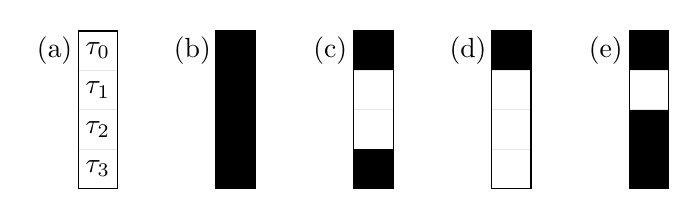
\begin{tikzpicture}[x=0.5cm, y=0.5cm] % {{{
\pgfmathsetmacro{\unitstep}{3.5}
% Coordenadas   {{{
\node at (-0.6,0.5) {(a)} ;
\draw[black!10] (0,0) rectangle (1,1); \node at (0.5,0.5) {$\tau_0$} ;
\begin{scope}[shift={(0,-1)}]
\draw[black!10] (0,0) rectangle (1,1); \node at (0.5,0.5) {$\tau_1$} ;
\end{scope}
\begin{scope}[shift={(0,-2)}]
\draw[black!10] (0,0) rectangle (1,1); \node at (0.5,0.5) {$\tau_2$} ;
\end{scope}
\begin{scope}[shift={(0,-3)}]
\draw[black!10] (0,0) rectangle (1,1); \node at (0.5,0.5) {$\tau_3$} ;
\end{scope} 
\draw (0,-3) rectangle (1,1); 
% }}}
\begin{scope}[shift={(1*\unitstep,0)}] % Identity {{{
% \begin{scope}[shift={(\unitstep*2,0)}]
\node at (-0.6,0.5) {(b)} ;
\fill[black] (0,0) rectangle (1,1);
\draw[black!10] (0,0) rectangle (1,1);
\begin{scope}[shift={(0,-1)}] \draw[black!10] (0,0) rectangle (1,1); \end{scope}
\begin{scope}[shift={(0,-2)}] \draw[black!10] (0,0) rectangle (1,1); \end{scope}
\begin{scope}[shift={(0,-3)}] \draw[black!10] (0,0) rectangle (1,1); \end{scope}
\draw (0,-3) rectangle (1,1); 
\begin{scope}[shift={(0,-1)}] \fill[black] (0,0) rectangle (1,1); \end{scope}
\begin{scope}[shift={(0,-2)}] \fill[black] (0,0) rectangle (1,1); \end{scope}
\begin{scope}[shift={(0,-3)}] \fill[black] (0,0) rectangle (1,1); \end{scope}
\end{scope} % }}}
\begin{scope}[shift={(2*\unitstep,0)}] % Dephasing {{{
\node at (-0.6,0.5) {(c)} ;
\fill[black] (0,0) rectangle (1,1);
% \draw (0,0) rectangle (1,1);
\draw[black!10] (0,0) rectangle (1,1);
\begin{scope}[shift={(0,-1)}] \draw[black!10] (0,0) rectangle (1,1); \end{scope}
\begin{scope}[shift={(0,-2)}] \draw[black!10] (0,0) rectangle (1,1); \end{scope}
\begin{scope}[shift={(0,-3)}] \draw[black!10] (0,0) rectangle (1,1); \end{scope}
\draw (0,-3) rectangle (1,1); 
% \begin{scope}[shift={(0,-1)}] \fill[black] (0,0) rectangle (1,1); \end{scope}
% \begin{scope}[shift={(0,-1)}] \draw (0,0) rectangle (1,1); \end{scope}
% \begin{scope}[shift={(0,-2)}] \fill[black] (0,0) rectangle (1,1); \end{scope}
% \begin{scope}[shift={(0,-2)}] \draw (0,0) rectangle (1,1); \end{scope}
\begin{scope}[shift={(0,-3)}] \fill[black] (0,0) rectangle (1,1); \end{scope}
% \begin{scope}[shift={(0,-3)}] \draw (0,0) rectangle (1,1); \end{scope}
\end{scope} % }}}
\begin{scope}[shift={(3*\unitstep,0)}] % Depolarization {{{
\node at (-0.6,0.5) {(d)} ;
\fill[black] (0,0) rectangle (1,1);
% \draw (0,0) rectangle (1,1);
\draw[black!10] (0,0) rectangle (1,1);
\begin{scope}[shift={(0,-1)}] \draw[black!10] (0,0) rectangle (1,1); \end{scope}
\begin{scope}[shift={(0,-2)}] \draw[black!10] (0,0) rectangle (1,1); \end{scope}
\begin{scope}[shift={(0,-3)}] \draw[black!10] (0,0) rectangle (1,1); \end{scope}
\draw (0,-3) rectangle (1,1); 
% \begin{scope}[shift={(0,-1)}] \fill[black] (0,0) rectangle (1,1); \end{scope}
% \begin{scope}[shift={(0,-1)}] \draw (0,0) rectangle (1,1); \end{scope}
% \begin{scope}[shift={(0,-2)}] \fill[black] (0,0) rectangle (1,1); \end{scope}
% \begin{scope}[shift={(0,-2)}] \draw (0,0) rectangle (1,1); \end{scope}
% \begin{scope}[shift={(0,-3)}] \fill[black] (0,0) rectangle (1,1); \end{scope}
% \begin{scope}[shift={(0,-3)}] \draw (0,0) rectangle (1,1); \end{scope}
\end{scope} % }}}
\begin{scope}[shift={(4*\unitstep,0)}] % (e) canal malo {{{
\node at (-0.6,0.5) {(e)} ;
\fill[black] (0,0) rectangle (1,1);
% \draw (0,0) rectangle (1,1);
\draw[black!10] (0,0) rectangle (1,1);
\begin{scope}[shift={(0,-1)}] \draw[black!10] (0,0) rectangle (1,1); \end{scope}
\begin{scope}[shift={(0,-2)}] \draw[black!10] (0,0) rectangle (1,1); \end{scope}
\begin{scope}[shift={(0,-3)}] \draw[black!10] (0,0) rectangle (1,1); \end{scope}
% \begin{scope}[shift={(0,-1)}] \fill[black] (0,0) rectangle (1,1); \end{scope}
% \begin{scope}[shift={(0,-1)}] \draw (0,0) rectangle (1,1); \end{scope}
\begin{scope}[shift={(0,-2)}] \fill[black] (0,0) rectangle (1,1); \end{scope}
% \begin{scope}[shift={(0,-2)}] \draw (0,0) rectangle (1,1); \end{scope}
\begin{scope}[shift={(0,-3)}] \fill[black] (0,0) rectangle (1,1); \end{scope}
% \begin{scope}[shift={(0,-3)}] \draw (0,0) rectangle (1,1); \end{scope}
\draw (0,-3) rectangle (1,1); 
\end{scope} % }}}
\end{tikzpicture} % }}}
\end{center}
	\caption{
% \janote{Le modificamos la primera frase a esta caption para que la Fig sea
% 	autocontenida}
In (a) we introduce the notation
in the diagrams that represent the single qubit \pce{} maps,
so that each square corresponds to a single 
$\tau_{\alpha}$, $\alpha=0,1,2,3$. The diagrams in 
(b), (c) and (d) correspond to the identity map, dephasing channel, and 
total depolarization, respectively, 
as the color of each square indicates the value attained by the corresponding
$\tau_{\alpha}$, either 0 (white) or 1 (black). 
In (e) we show a map that only erases the component
$r_1$, collapsing the Bloch sphere into a disk, and thus does not correspond to
a quantum operation.
% \afnote{Propongo el siguiente caption: (a) Pictorial
% representation of a single qubit \pce{} map.
% The color of each square indicates the value attained by the corresponding
% $\tau_{\alpha}$, either 0 (white) or 1 (black). The diagrams in (b), (c) and
% (d) correspond to the identity map, dephasing channel, and total
% depolarization, respectively. In (e) we show a map that only erases the
% component $r_1$, collapsing the Bloch sphere into a disk, and thus does not
% correspond to a quantum operation.}
}
	\label{fig:one:qubit:examples}
\end{figure} % }}}
% }}}
% \subsection{$\mathbf{N}$ qubits Pauli component erasing maps} % {{{


In order to present and develop the $N$ qubit case, it is useful 
to introduce 
the so-called \textit{Pauli strings}, defined as 
\begin{equation}
\sigma_{\vec \alpha}=\sigma_{\alpha_1}\otimes \sigma_{\alpha_2} \otimes \dots \otimes \sigma_{\alpha_N},
\label{eq:pauli_strings}
\end{equation}
where $\vec \alpha$ denotes a multi-index $\qty(\alpha_1,\ldots,\alpha_N)$
\janote{revisar si en el resto del artículo siempre le llamamos a $\valpha$
`vector index'. A veces le poníamos `multi-index'}
and $\alpha_i=0,1,2,3$. These hermitian operators form an orthogonal 
basis in the space of operators acting on $N$ qubits. In fact, 
$\tr \sigma_{\vec \alpha} \sigma_{\vec \alpha'}=2^N\delta_{\valpha \valpha'}$
and 
$\tr \sigma_{\vec \alpha}= 2^{N}\delta_{\vec\alpha \vec 0}$.
% 
% Thus, given $N$ and the fact that $\tr
% \sigma_{\vec \alpha}=\delta_{\vec\alpha,\vec 0} 2^{N}$, it is clear that the
% basis $\left\{ 2^{N/2} \sigma_{\vec \alpha} \right\}$ is orthonormal in
% $\mcB(\hilbert_{2^N})$. The case with $N=1$ corresponds to the well-known
% \textit{Pauli basis},
% $1/\sqrt{2} \left\{ \one, \sigma_x,\sigma_y,\sigma_z \right\}$.


Similarly to the single qubit case, the density matrix $\rho$ of a system of $N$
qubits can be written using Pauli strings in the following way, 
\begin{equation}\label{eq:N_qubits_rho}
	\rho =\frac{1}{2^N} 
            \sum_\valpha r_\valpha \sigma_\valpha,
%             \quad r_{\vec0}=1,
% 	\sigma_{\alpha_1}\otimes \ldots \otimes \sigma_{\alpha_N},
%             \sum_{\alpha_1,\ldots,\alpha_N=0}^3 \paulicomponents
% 	\sigma_{\alpha_1}\otimes \ldots \otimes \sigma_{\alpha_N},
	%r_{0,\ldots,0}=1,
\end{equation}
so $r_{\vec \alpha}=\langle \sigma_{\vec \alpha} \rangle=\tr \left(\rho
\sigma_{\vec \alpha} \right)$ is the coefficient corresponding to the expansion
of the density matrix in the normalized basis of Pauli strings.  Again,
normalization of the state requires that $r_{\vec 0}=1$.
We shall refer to $\paulicomponents$ as the {\it Pauli components} of the density
matrix of a system of qubits. 

% The components of $\valpha$ range from $0$ to $3$.  Notice that
% given that $\tr \rho=1$ and $\sigma_{\vec 0} = \openone$, it is clear that
% $r_{\vec 0}=1$. Additionally, observe that $\vec r_{\vec \alpha}$ can be
% understood as a generalization of the Bloch vector for $N$ qubits.
% 



% The density matrix $\rho$ of a system of $N$ qubits can be written in Pauli
% matrices basis as 
% \begin{equation}\label{eq:N_qubits_rho}
% 	\rho =\frac{1}{2^N} 
%             \sum_\valpha r_\valpha \sigma_\valpha,
% %             \quad r_{\vec0}=1,
% % 	\sigma_{\alpha_1}\otimes \ldots \otimes \sigma_{\alpha_N},
% %             \sum_{\alpha_1,\ldots,\alpha_N=0}^3 \paulicomponents
% % 	\sigma_{\alpha_1}\otimes \ldots \otimes \sigma_{\alpha_N},
% 	%r_{0,\ldots,0}=1,
% \end{equation}
% where $\vec \alpha$ denotes a vector index $\qty(\alpha_1,\ldots,\alpha_N)$,
% $\sigma_{\vec \alpha} := \sigma_{\alpha_1}\otimes \ldots \otimes
% \sigma_{\alpha_N}$ is the tensor product of Pauli matrices, and 
% $r_{\vec \alpha}$ is the coefficient corresponding to the expansion
% of the density matrix in the complete orthonormal basis $\left\{ 2^{-N/2}\sigma_{\vec
% \alpha} \right\}$. In the sum each of the $N$ components of $\valpha$, i.e.
% $\alpha_{1,\cdots,N}$ is varied from $0$ to $3$. 
% Notice that $\sigma_{\vec 0} = \openone$, and since both $\tr \rho=1$ and 
% $\tr \sigma_\valpha=2^N\delta_{\valpha,\vec 0}$, then $r_{\vec 0}=1$. 
% We shall refer to $\paulicomponents$ as the ``Pauli components'' of the density
% matrix of a system of qubits. 


% Thus, i
In general, a Pauli component erasing (PCE) map is a map
%  Pauli diagonal operation
that either preserves or completely erases the Pauli components of a
density matrix. That is, 
% it transforms its Pauli components as 
\begin{equation} \label{eq:PCE_definition}
% \begin{split}
% 	\paulicomponents \mapsto \ \taus \paulicomponents,\hspace{.5cm}\\
% 	\taus = 0,1, \hspace{1.5cm}	\tau_{0,\ldots,0}=1.
	\paulicomponents \mapsto \taus \paulicomponents,\quad 
	\taus = 0,1.
% \end{split}
\end{equation}
In addition, for the operation to be trace preserving, it is required that $\tau_{\vec
0}=1$. 
It is worth noticing that, as for the single qubit case, not all PCE maps are
quantum operations. 
On the other hand, constructing and
evaluating the conditions for complete positivity is non-trivial and is the main
problem addressed in this paper.
We shall refer to the map  $\paulicomponents \mapsto \taus \paulicomponents$, 
with arbitrary values of 
% but allow the 
$\taus$ (only restricted by complete positivity) as {\it Pauli diagonal operations}. 


% For single 
% qubits, if just one of the $\taus=0$, the complete positivity condition 
% is not met, as discussed in \sref{sec:single:qubit}. 
% It will be of central interest
% in this article to determine which $\taus$ lead to a valid quantum map.


% On the other hand, constructing and
% evaluating the conditions for complete positivity is involved and is the main
% problem addressed in this paper. 
% Moreover, these operations are by definition
% diagonal in the $\left\{ 2^{-N/2}\sigma_{\vec
% \alpha} \right\}$ basis.


% As mentioned above, \pce{} maps\R{A1} nullify Pauli strings, thus, consider the linear operations acting in the generalized Bloch vector $\vec r_{\vec \alpha}$,
% \begin{equation}
% 	\paulicomponents \mapsto \taus \paulicomponents.
% % 	\taus = 0,1, \hspace{1.5cm}	\tau_{0,\ldots,0}=1,
% \label{eq:definition:Pauli}
% \end{equation}
% % with $\tau_{\vec \alpha}$ either $1$ or $0$.
% % \cpnote{Revisar aca lo que sigue}
% % Similar to the qubit case, not every operation with this form is a completely
% % positive trace perserving map. 
% For the operation to be trace preserving, it is
% easy to prove that $\tau_{\vec 0}=1$. On the other hand, constructing and
% evaluating the conditions for complete positivity is involved and is the main
% problem addressed in this paper. Moreover, these operations are by definition
% diagonal in the $\left\{ 2^{-N/2}\sigma_{\vec
% \alpha} \right\}$ basis.

% \cpnote{Creo qeu vale la pena mencionar la relacion con los canales de Ruskai.
% Lo discutimos en pleno, o por lo menos cuando esten JA y FL. quizá tambien
% discutir si se mencionan a los canales  \cite{Siudzinska2020}}\ddnote{Eh estado
% trabajando en esto, pero el material que he encontrado va mejor en la
% introduccion, y en todo caso, creo que es muy pronto para mencionar detalles
% tecnicos sobre los canales que coinciden con los de Ruskai, pues ni siquiera
% hemos dicho que operaciones de las que definimos aqui, son válidas}

A graphical representation for PCE maps may be introduced, being the
two qubits case what has proved to be the most useful. Consider a $N$ dimensional 
Cartesian grid, with $4^N$ places.  Each place has $N$ integer coordinates, ranging
from 0 to 3, so each place corresponds to a given $\vec \alpha$ in 
\eref{eq:N_qubits_rho}. For a given PCE, we shall fill  
the square if the corresponding $\tau_{\vec \alpha}=1$. Otherwise, we leave it 
empty. 
Examples for $N=1$ and $N=2$ are provided in \fref{fig:one:qubit:examples} and
\fref{fig:two:qubit:examples}, respectively.




It is worth noticing that the set of \pce{} maps overlaps with the set
of ``Pauli diagonal channels constant on axes'' defined in
Ref.~\cite{nathanson2007pauli}, consisting of convex combinations of
\textit{quantum-classical} channels. In particular, it can be shown that
quantum-classical channels defined with the eigenbasis of some set of $2^N-1$
commuting Pauli observables~\cite{Lawrence2002}, is a \pce{} map with exactly $
2^N $ components equal to $1$s in its diagonal.
% \afnote{Aquí me parece que falta información. Creo que hay que decir que es lo
% que es diagonal y en que base.} 
For details, we refer the reader to appendix~\ref{quantum_classical}.


% \cpnote{davalos, dale aca un pequeño rollo relevante quiza de una o dos
% frases de la importancia de esta familia.} \ddnote{hecho, pero de pronto
% quedo espeso. Me estan gustando las cosas que he estado encontrando, voy a
% investigar en esa direccion por mi cuenta, si sale algo interesante, los
% invito, como no}
% 
%\ddnote{hay un typo en esta ecuacion}
% A PCE operation is a trace-preserving operation that leaves invariant or erases 
% the Pauli components of a density matrix of $n$ qubits. \janote{Ojo que aquí 
% habrá que unificar la notación de subíndices. No lo hago porque no lo tengo del 
% todo claro y no hay problema en dejarlo así por el momento.}
% \cpnote{Aca voy} 

% For the two qubits case, the operations illustrated
% in~\eref{eq:definition:Pauli} can be pictured using $4\times 4$ tables, showing
% the positions of the $0$s and $1$s of the diagonal using the Pauli string
% basis, see~\fref{fig:two:qubit:examples}. This way of representing \pce{}
% maps\R{A3} turned out to be very useful for their analysis throughout this
% work.
% 


% Notice
% than in both cases we drop the label $\alpha$ for simplicity, as it will 
% remain unchanged throughout this text \janote{No entiendo qué estás diciendo
% aquí}. 



\begin{figure} % {{{
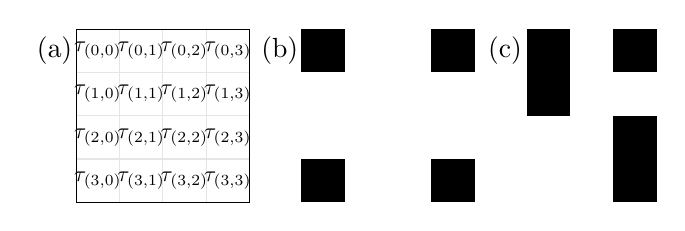
\begin{tikzpicture}[x=0.55cm, y=0.55cm] % {{{
\pgfmathsetmacro{\unitstep}{5.2}
\begin{scope}[shift={(0*\unitstep,0)}] % Coordenadas {{{
\node at (-0.5,0.5) {(a)} ;
% \cuadritotikz{}
    \foreach \x in {0,1,2,3} {
      \foreach \y in {0,1,2,3} {
        \begin{scope}[shift={(\x,-\y)}] 
          \draw[black!10] (0,0) rectangle (1,1); 
%           \draw (0,0) rectangle (1,1); 
          \node at (0.5,0.5) {\scalebox{.8}{$\tau_{(\y,\x)}$}};
         \end{scope}
%         \node at (0,-\y) (input\y) {$i_\y$};
%         \node[block] at (2,-\y) (block\y) {$f_\y$};
%         \draw[->] (input\y) -- (block\y);
%         \draw[->] (block\y.east) -- +(0.5,0);
    }
    }
 \draw (0,-3) rectangle (4,1);
\end{scope} % }}}
\begin{scope}[shift={(1*\unitstep,0)}] % Good channel {{{
\node at (-0.5,0.5) {(b)} ;
\cuadritotikz{}
%     \foreach \x in {0,1,2,3} {
%       \foreach \y in {0,1,2,3} {
%         \begin{scope}[shift={(\x,-\y)}] 
%           \draw (0,0) rectangle (1,1); 
% %           \node at (0.5,0.5) {$\tau_{\y,\x}$};
%          \end{scope}
% %         \node at (0,-\y) (input\y) {$i_\y$};
% %         \node[block] at (2,-\y) (block\y) {$f_\y$};
% %         \draw[->] (input\y) -- (block\y);
% %         \draw[->] (block\y.east) -- +(0.5,0);
%     }
%     }
\begin{scope}[shift={(0,-3)}] \fill[black] (0,0) rectangle (1,1); \end{scope}
\begin{scope}[shift={(3,-3)}] \fill[black] (0,0) rectangle (1,1); \end{scope}
\begin{scope}[shift={(0,0)}] \fill[black] (0,0) rectangle (1,1); \end{scope}
\begin{scope}[shift={(3,0)}] \fill[black] (0,0) rectangle (1,1); \end{scope}
\end{scope} % }}}
\begin{scope}[shift={(2*\unitstep,0)}] % Good channel {{{
\node at (-0.5,0.5) {(c)} ;
\cuadritotikz{}
%     \foreach \x in {0,1,2,3} {
%       \foreach \y in {0,1,2,3} {
%         \begin{scope}[shift={(\x,-\y)}] 
%           \draw (0,0) rectangle (1,1); 
% %           \node at (0.5,0.5) {$\tau_{\y,\x}$};
%          \end{scope}
% %         \node at (0,-\y) (input\y) {$i_\y$};
% %         \node[block] at (2,-\y) (block\y) {$f_\y$};
% %         \draw[->] (input\y) -- (block\y);
% %         \draw[->] (block\y.east) -- +(0.5,0);
%     }
%     }
\begin{scope}[shift={(0,0)}] \fill[black] (0,0) rectangle (1,1); \end{scope}
\begin{scope}[shift={(0,-1)}] \fill[black] (0,0) rectangle (1,1); \end{scope}
\begin{scope}[shift={(2,0)}] \fill[black] (0,0) rectangle (1,1); \end{scope}
\begin{scope}[shift={(2,-2)}] \fill[black] (0,0) rectangle (1,1); \end{scope}
\begin{scope}[shift={(2,-3)}] \fill[black] (0,0) rectangle (1,1); \end{scope}
\end{scope} % }}}
\end{tikzpicture} % }}}
	\caption{In (a) we introduce the
positions of two qubit diagrams. The diagrams in 
(b) corresponds to a quantum channel that results from the tensor product of
bit flip channels in each qubit [see \fref{fig:one:qubit:examples}(c)],
and in (c) a diagram of a map that is not a quantum channel is presented.}
	\label{fig:two:qubit:examples}
\end{figure} % }}}

% In \Fref{fig:PCE_figs} we introduce a pictorial representation of PCE operations of 
% 1, 2 and 3 qubits. Every position in the column, board or cube is associated with 
% the subindices of $\taus$ of a PCE operation. If a little square or cube  in position
% $\alpha_1,\ldots,\alpha_N$ is black, then $\taus=1$, if it is white, then $\taus=0$. For example,
% \begin{center}
% 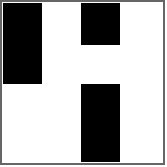
\includegraphics[width=2cm]{2qubits_pce_example}
% \end{center}
% this represents a PCE operation of 2 qubits that leaves invariant the Pauli 
% components $r_{0,0}$, $r_{0,2}$, $r_{1,0}$, $r_{2,2}$, $r_{3,2}$. This operation
% is not completely positive and therefore is not a quantum channel. In contrast, 
% \begin{center}
% \includegraphics[width=2cm]{2qubits_pceChannel_example01}
% \end{center}
% this other example of PCE operation that leaves invariant Pauli components 
% $r_{0,0}$, $r_{1,2}$, $r_{2,1}$, $r_{3,3}$ satisfies complete positivity and 
% is a quantum channel. 
% 
% 



% }}}




